% System / implementation architecture -- ROS nodes and topics as actually wired
% (state after the rosification merge, 2026-07-18). Solid arrows = ROS topics,
% dashed = direct in-process calls; blue = ROS node, gray = plain object.
% Compile: pdflatex system_architecture.tex
\documentclass[tikz,border=10pt]{standalone}
\usetikzlibrary{positioning,fit,arrows.meta,backgrounds,calc}

\definecolor{nodeblue}{RGB}{31,119,180}
\definecolor{extgray}{RGB}{110,110,110}
\definecolor{goalgreen}{RGB}{34,120,44}

\begin{document}
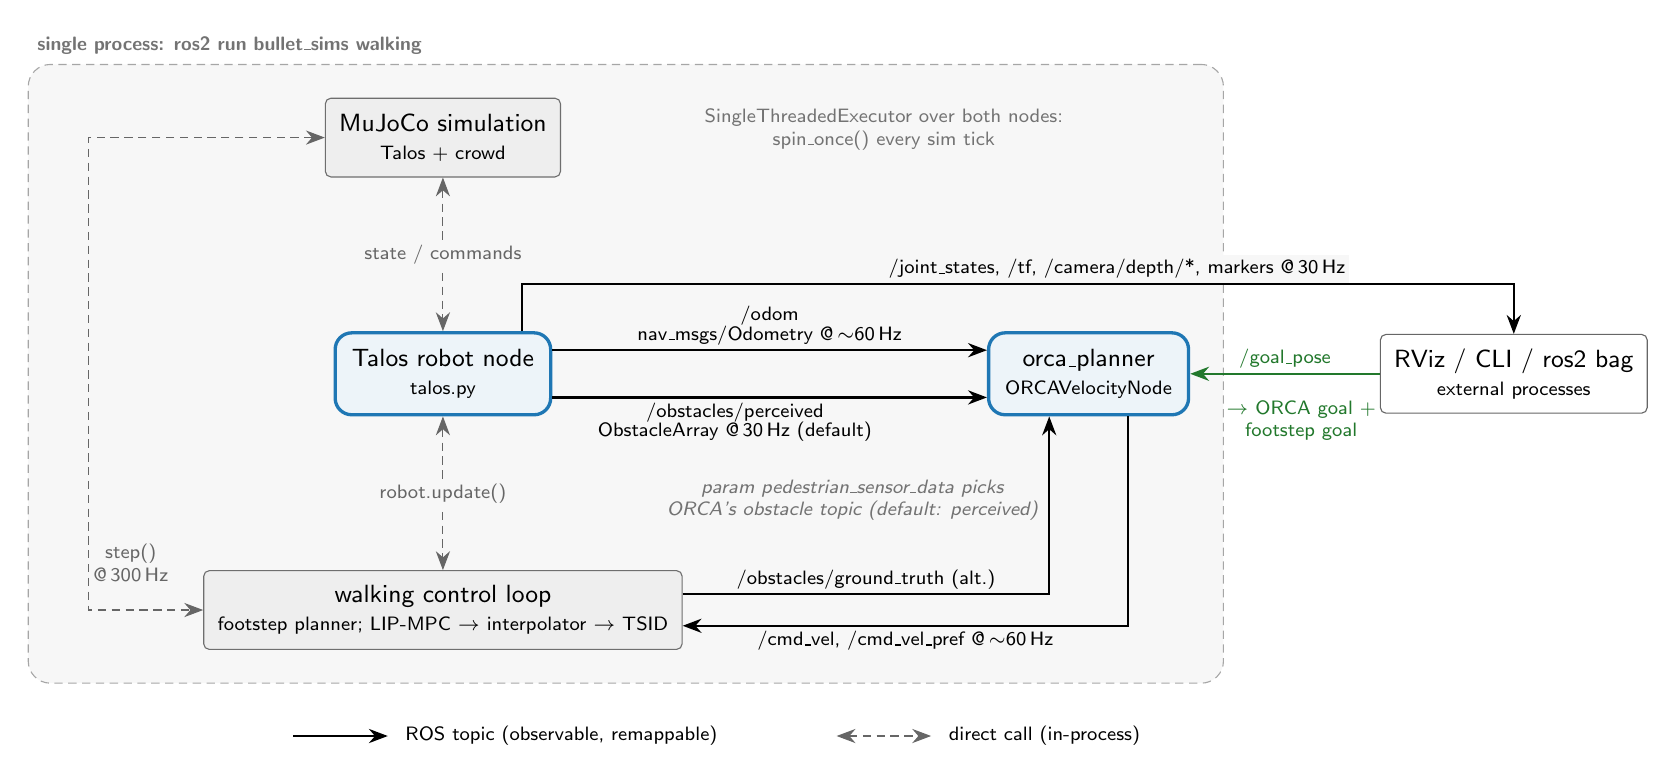
\begin{tikzpicture}[
  font=\sffamily\small,
  >={Stealth[length=2.4mm]},
  rosnode/.style={draw=nodeblue, very thick, rounded corners=6pt, align=center,
                  minimum height=10mm, inner sep=6pt, fill=nodeblue!8},
  plain/.style={draw=extgray, rounded corners=2pt, align=center,
                minimum height=10mm, inner sep=5pt, fill=extgray!12},
  external/.style={draw=black!60, rounded corners=2pt, align=center,
                   minimum height=10mm, inner sep=5pt, fill=white},
  topic/.style={->, thick},
  direct/.style={<->, densely dashed, black!60},
  lab/.style={font=\sffamily\scriptsize, align=center, fill=black!3, inner sep=1.5pt},
  labw/.style={font=\sffamily\scriptsize, align=center, fill=white, inner sep=1.5pt},
]

% ---------------- in-process components ----------------
\node[plain]   (sim)   at (0,0)    {MuJoCo simulation\\[-1pt]\scriptsize Talos + crowd};
\node[rosnode] (talos) at (0,-3)   {Talos robot node\\[-1pt]\scriptsize talos.py};
\node[plain]   (loop)  at (0,-6)   {walking control loop\\[-1pt]\scriptsize footstep planner; LIP-MPC $\to$ interpolator $\to$ TSID};
\node[rosnode] (orca)  at (8.2,-3) {orca\_planner\\[-1pt]\scriptsize ORCAVelocityNode};

% executor note
\node[font=\sffamily\scriptsize, text=black!55, align=center] (exec) at (5.6,0.1)
     {SingleThreadedExecutor over both nodes:\\ spin\_once() every sim tick};

% ---------------- external ----------------
\node[external] (rviz) at (13.6,-3)
     {RViz / CLI / ros2 bag\\[-1pt]\scriptsize external processes};

% ---------------- process boundary ----------------
\coordinate (procpad) at ($(loop.west)+(-1.8,0)$);
\begin{scope}[on background layer]
  \node[rounded corners=8pt, draw=black!35, densely dashed, fill=black!3,
        inner sep=12pt, fit=(sim)(talos)(loop)(orca)(exec)(procpad)] (proc) {};
\end{scope}
\node[anchor=south west, font=\sffamily\scriptsize\bfseries, text=black!55]
     at (proc.north west) {single process: ros2 run bullet\_sims walking};

% ---------------- direct (in-process) calls ----------------
\draw[direct] (sim)   -- node[lab]{state / commands} (talos);
\draw[direct] (talos) -- node[lab]{robot.update()} (loop);
\draw[direct] (sim.west) -- ++(-3.0,0) |-
              node[lab, right, pos=0.45, align=center]{step()\\@\,300\,Hz} (loop.west);

% ---------------- topics: robot node -> orca ----------------
\draw[topic] ($(talos.east)+(0,0.3)$) -- node[lab, above, pos=0.5]
     {/odom\\[-1pt]nav\_msgs/Odometry @\,$\sim$60\,Hz} ($(orca.west)+(0,0.3)$);
\draw[topic] ($(talos.east)+(0,-0.3)$) -- node[lab, below, pos=0.42]
     {/obstacles/perceived\\[-1pt]ObstacleArray @\,30\,Hz (default)} ($(orca.west)+(0,-0.3)$);

% ---------------- topics: loop <-> orca ----------------
\draw[topic] ($(loop.east)+(0,0.2)$) -| node[lab, above, pos=0.25]
     {/obstacles/ground\_truth (alt.)} ($(orca.south)+(-0.5,0)$);
\draw[topic] ($(orca.south)+(0.5,0)$) |- node[lab, below, pos=0.75]
     {/cmd\_vel, /cmd\_vel\_pref @\,$\sim$60\,Hz} ($(loop.east)+(0,-0.2)$);

% mode-selection note
\node[font=\sffamily\scriptsize\itshape, text=black!55, align=center]
     at (5.2,-4.6) {param pedestrian\_sensor\_data picks\\ ORCA's obstacle topic (default: perceived)};

% ---------------- topics: to/from external ----------------
\draw[topic, goalgreen] (rviz.west) -- node[labw, above]
     {/goal\_pose} (orca.east);
\node[font=\sffamily\scriptsize, text=goalgreen, align=center]
     at (10.9,-3.6) {$\to$ ORCA goal +\\ footstep goal};

\draw[topic] ($(talos.north)+(1.0,0)$) -- ++(0,0.6) -| node[lab, above, pos=0.3]
     {/joint\_states, /tf, /camera/depth/*, markers @\,30\,Hz} (rviz.north);

% ---------------- legend ----------------
\draw[topic] (-1.9,-7.6) -- (-0.7,-7.6);
\node[anchor=west, font=\sffamily\scriptsize] at (-0.6,-7.6) {ROS topic (observable, remappable)};
\draw[direct] (5.0,-7.6) -- (6.2,-7.6);
\node[anchor=west, font=\sffamily\scriptsize] at (6.3,-7.6) {direct call (in-process)};
%\node[rosnode, minimum height=4.5mm, minimum width=8mm, inner sep=1pt] at (10.4,-8.6) {};
%node[anchor=west, font=\sffamily\scriptsize] at (10.9,-8.6) {ROS node};
%node[plain, minimum height=4.5mm, minimum width=8mm, inner sep=1pt] at (12.9,-8.6) {};
%\node[anchor=west, font=\sffamily\scriptsize] at (13.4,-8.6) {plain object};

\end{tikzpicture}
\end{document}
